\chapter{Experiments}
This chapter will experiments that were performed to determine the performance of all the different algorithms, DQN, Double DQN and Duelling DQN. The three different environments are the three Atari games we have discussed before, that is, Pong, Breakout and Space Invaders. Each of the environments provides a different challenge, especially Space Invaders which proposed a unique challenge. This chapter also contains an analysis of the reasons why some of these methods are better performing than others which follows from the discussion in Section \ref{dsgn:sec:qlearning:qextra}.

\section{Atari Network}
This section will describe the choice of hyperparameters during training and additionaly motivate the choices to some of the hyperparameters that were chosen for the evaluation of the algorithms. The network architecture was descirbed completely in Section \ref{imple:cnn} and is also provided in a table in the table \ref{table:network-arch}. This architecture of the agent was used during the training of all the agents for all environments.

\begin{table}[htbp]
	\centering
	\begin{tabular}{|c|c|c|c|c|c|c|}
		\hline
		Layer   & Input    & Filter Size & \# Filters & Stride & Activation function & Output   \\ \hline
		conv\_1 & 4x84x84  & 20x20       & 32         & 4      & ReLU                & 32x20x20 \\
		conv\_2 & 32x20x20 & 9x9         & 64         & 2      & ReLU                & 64x9x9   \\
		conv\_3 & 64x9x9   & 7x7         & 64         & 1      & ReLU                & 64x7x7   \\
		fc\_1   & 64x7x7   & -           & -          & -      & ReLU                & 256      \\
		fc\_2   & 256      & -           & -          & -      & ReLU                & 4        \\ \hline
	\end{tabular}
	\caption{Table of the network architecture
		\label{table:network-arch}
	}
\end{table}

As has been noted previously, the output of the network is sometimes dependent on the game that is currently being trained. The final output varies between 4 and 6 nodes. Addition, the hyperparameters used for all the experiments in the following sections is provided in Appendix \ref{appen:train}. The only difference was in Space Invaders where the frameskip hyperparameter was set as $k = 3$ instead of the standard $k = 4$ as is used in Pong and Breakout.

\subsection{Pong}
Pong is the first environment which this project was trained using, it is by far the simplest of environments in the Atari 2600 series and provides an excellent testbed for RL algorithms. Due to the simplicity of the game, modern RL methods allows the algorithms to converge to an optimal strategy very quickly, therefore, it is easy to tell if an approach is viable or the implementation contains bugs that affect the performance of the agent.

During the training phase of Pong, it was tested using three methods, that is, DQN, Double and Duelling DQN.

\begin{figure}[htbp]
	\centering
	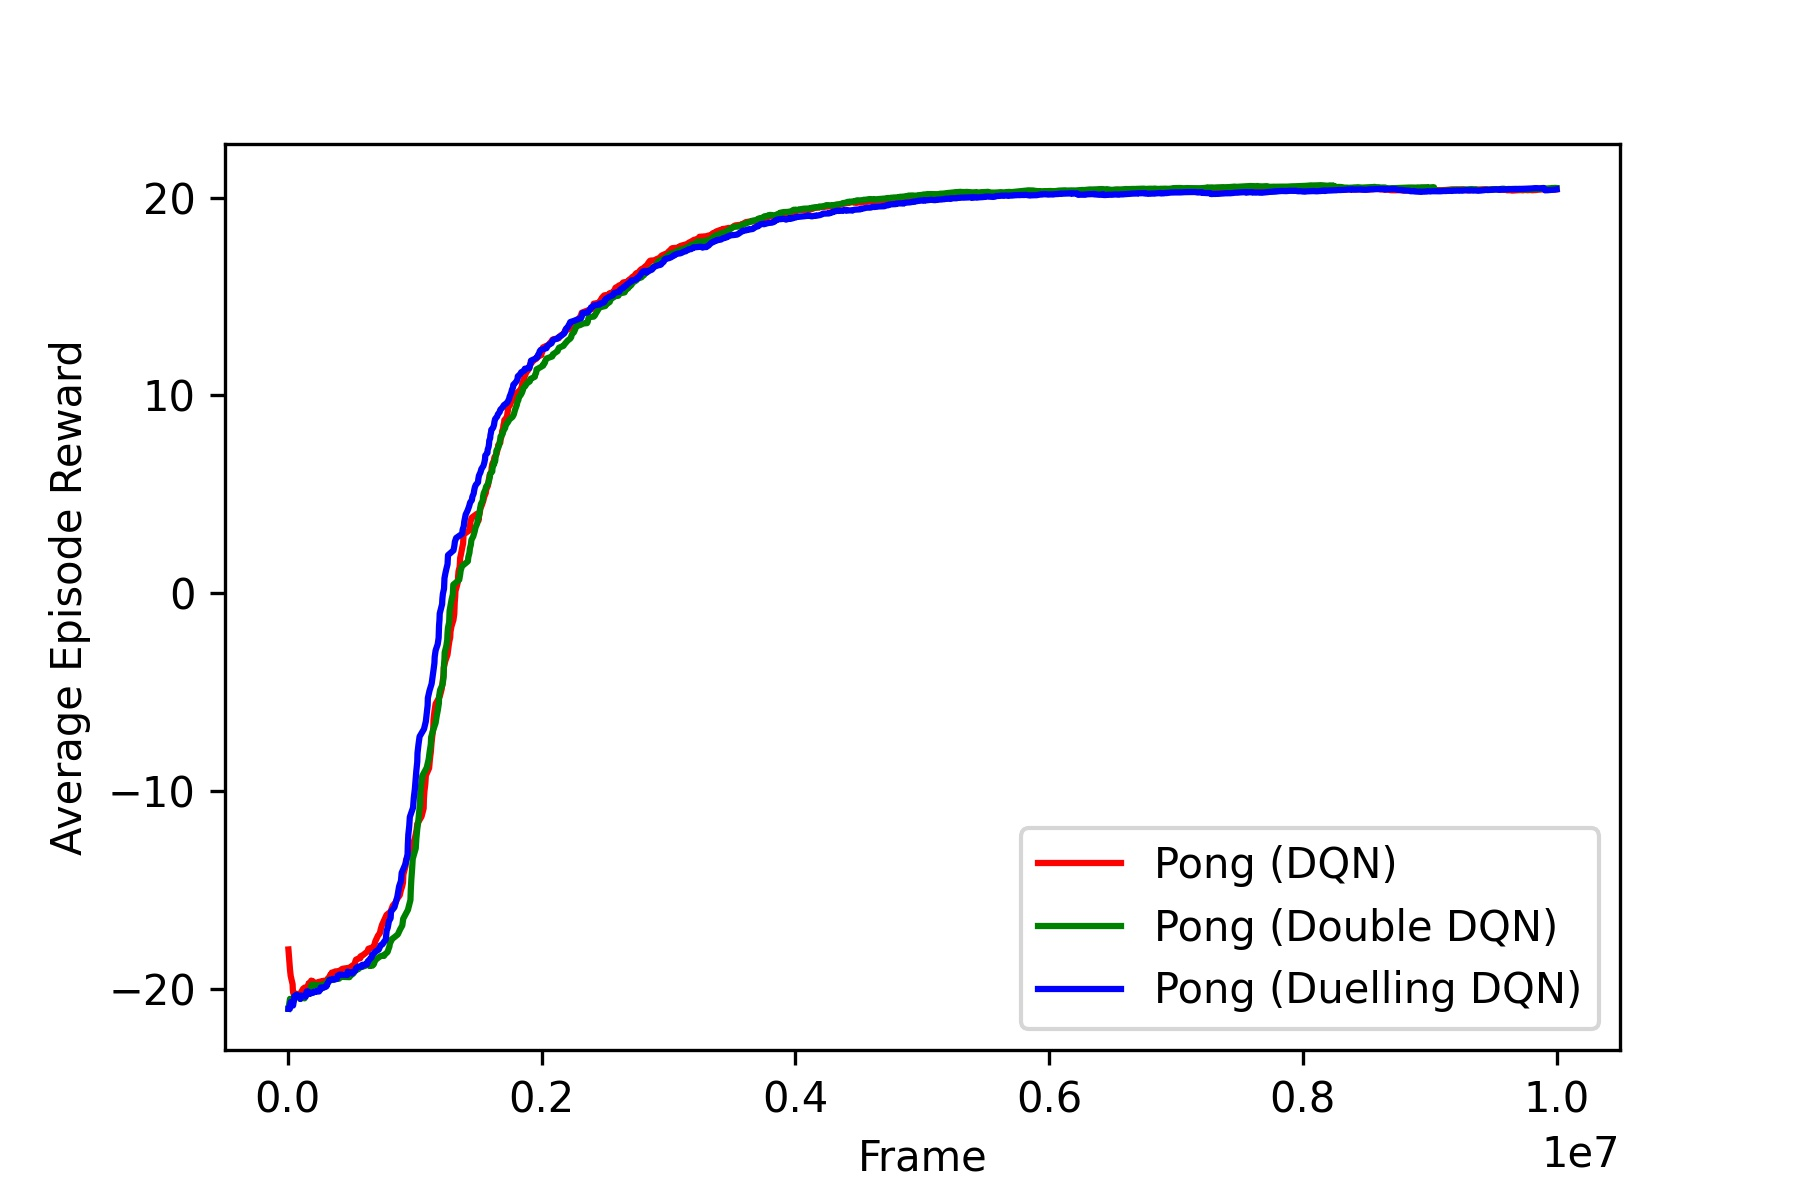
\includegraphics[width=0.75\textwidth]{chapters/chapter5/images/pong_plot.jpg}
	\caption[Pong Training results]{
		\label{fig:pong-train-results}
	}
\end{figure}

The agent was allowed to play a maximum of 10 million frames of Pong (Pong converges quickly, therefore it doesn't need the 20 million frames that other games like Breakout and Space Invaders require). Additionally, due to the limited compute power available to this project, a single Nvidia GTX 1070, training the agent for 20 million frames takes just over 24 hours. Therefore, the number of opportunities to perform  which results in approximately 6000 episodes\footnote{An episode is considered complete when the agent loses a life.}. Figure \ref{fig:pong-train-results} shows the results during training of the agent. This plot shows that all three algorithms result in a convergence plot reaching the threshold for the maximum score after less than 5 million frames. In this environment, non of the methods can be said to outperform the others, all the algorithms eventually converge to the best possible score of $+21$.

\subsection{Breakout}
Breakout was the second of the three environments upon which the agent was trained. We used the same network architecture as we did for Pong and the hyperparameters were the same during training with the exception of the number of timesteps for which the agent was trained. In Pong we used 10 million timesteps, however, since Breakout is more complex, it required 20 million timesteps to show a trend in the data that the agent is indeed improving over time. It should be noted that in the majority of papers that are referenced in this project it is common to use 100 million timesteps when training on Atari; it would not be feasible to train the agent for this number of timesteps on the hardware used for training as this would take over 5 days for a single algorithm on the environment.

\begin{figure}[htbp]
	\centering
	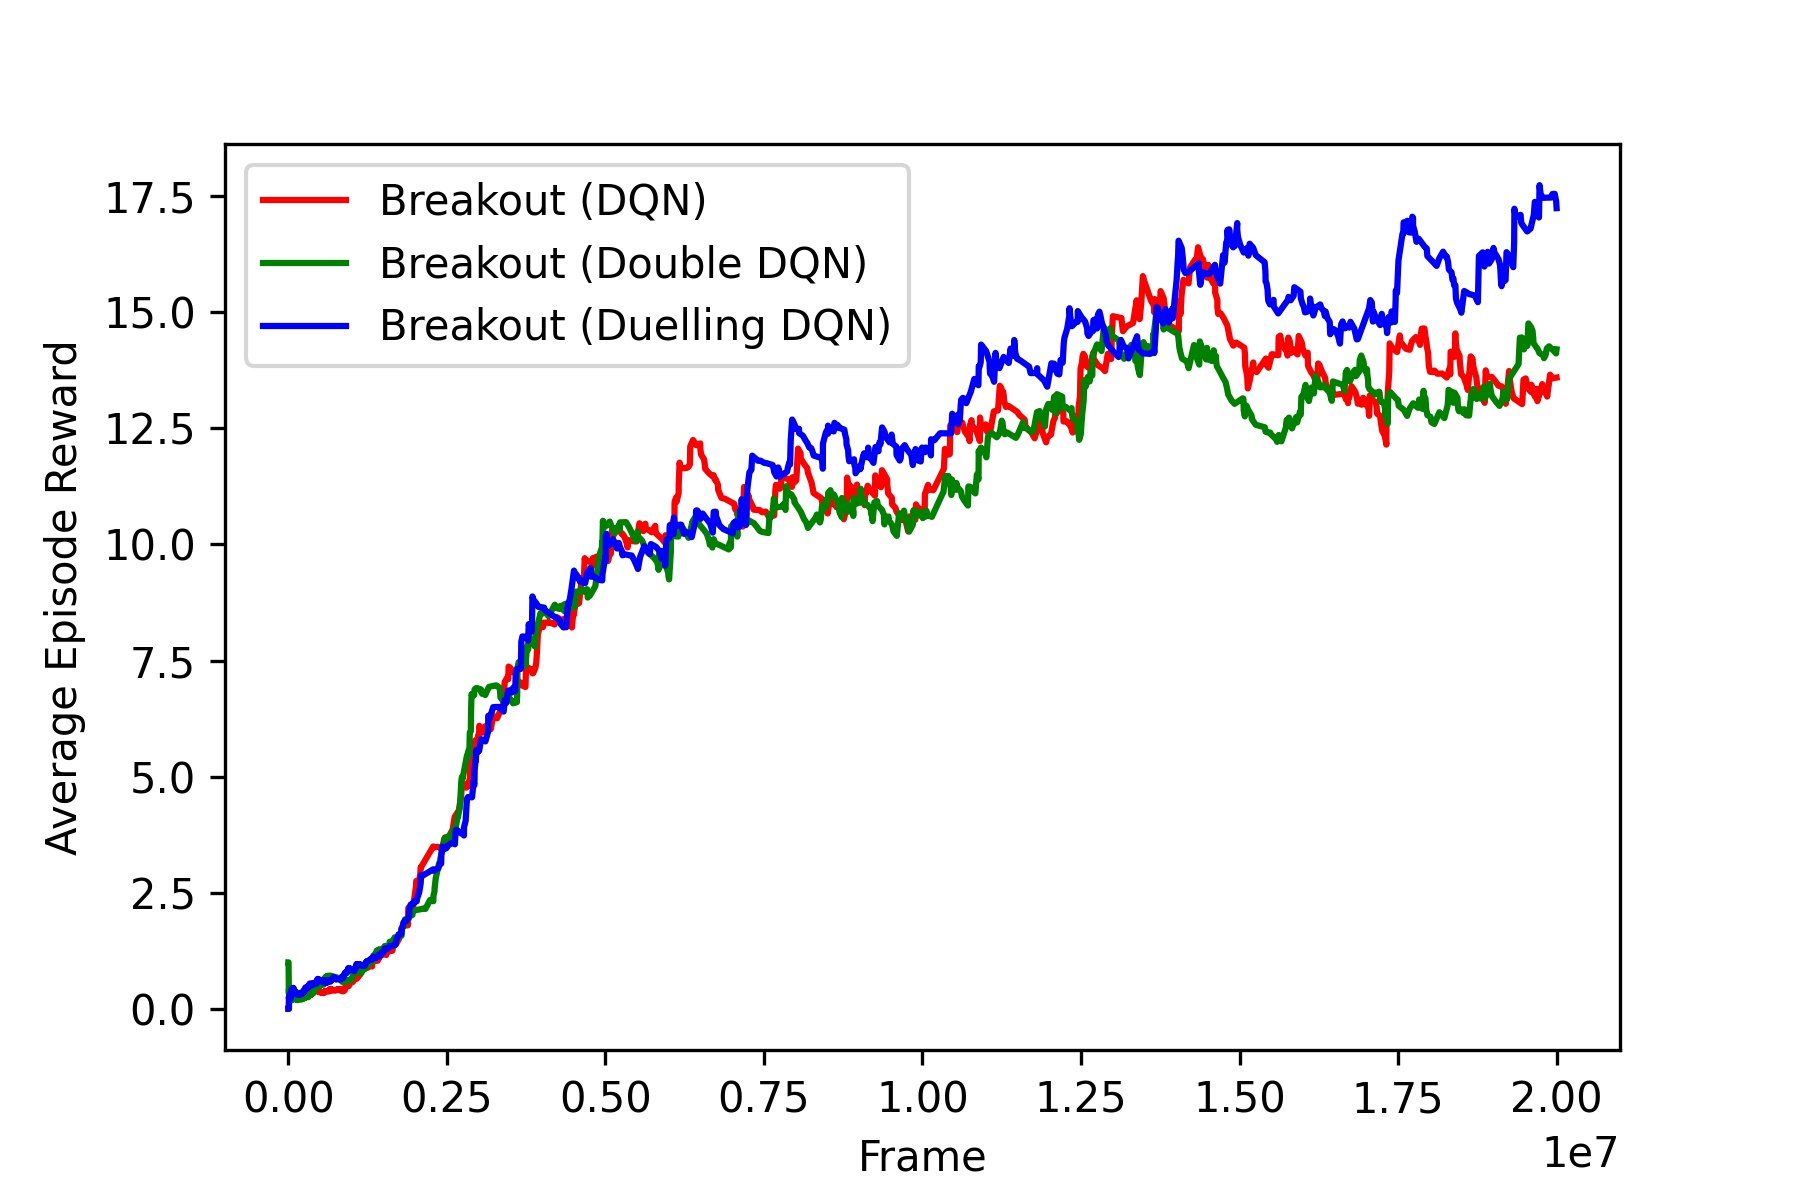
\includegraphics[width=0.75\textwidth]{chapters/chapter5/images/breakout_plot.jpg}
	\caption[Breakout Training results]{
		\label{fig:breakout-train-results}
	}
\end{figure}

Figure \ref{fig:breakout-train-results} shows the results of training the agent of 20 million timesteps, the plots are generated using a exponential weighted mean where the decay is expressed in terms of a window (span) 200 samples. The red, green and blue lines show the results for training the DQN, Double DQN and Duelling DQN respecitvely. We can clearly observe that the DQN algorithm is the worst performing with the duelling DQN having the most stable and best performance. We also observe the same results during evaluation of the different algorithms that is shown in Table \ref{table:eval:testing-results}.

\subsection{Space Invaders}
Space Invaders was the final and most difficult environment that the algorithms were trained upon. It presented some challenges during training, one notable challenge was that the \textit{``frameskip''} hyperparameter could not be kept at the value of $k = 4$ like was used in the previous two environments. In the Atari Space Invaders the players bullets flashed off every four frames. This meant that everytime the frame was sampled, we always missed the player bullet and therefore the agent would of needed to learn to play without the all the information about the players bullets. Therefore, for Space Invaders we changed to a frameskip of $k = 3$.

Figure \ref{fig:si-train-results} shows the results of the training the agent over a period of 20 million timesteps. We can observe from the training results that the Duelling DQN performed the best by the end of training, although the training was more gradual as compared to the standard and double DQN algorithms. We can conclude from the training results that the Duelling DQN, although it is slower to train (due to a more complex network architecture), it performs better than other methods and is more stable. We see more variance in the training results for the DQN algorithm especially after 5 million frames; a further investigation could be to implement a learning rate schedule which would reduce the learning rate after 5 million frames and observe if it results in more stability.

\begin{figure}[htbp]
	\centering
	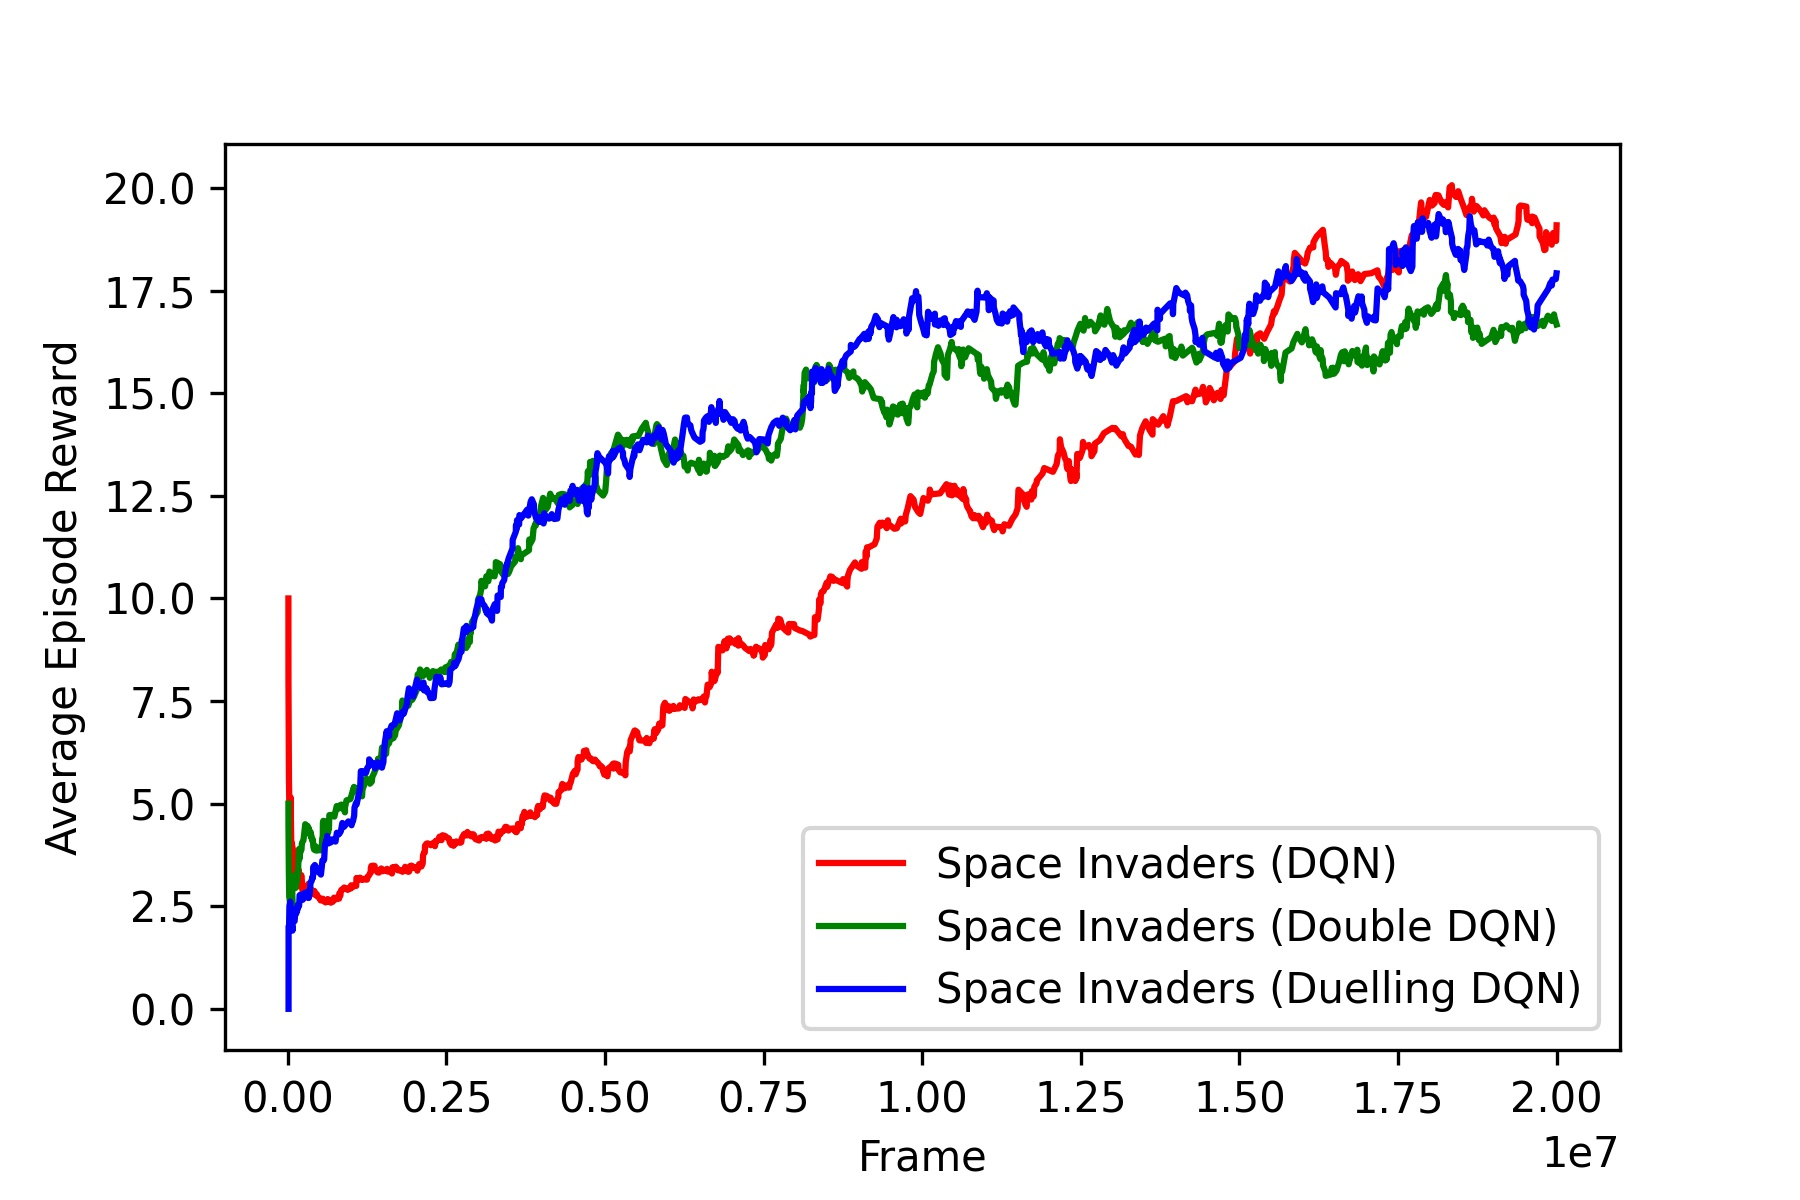
\includegraphics[width=0.75\textwidth]{chapters/chapter5/images/si_plot.jpg}
	\caption[Space Invaders training result plot]{Space Invaders training result. The results are shown for training on the three different algorithms which can be seen in the legend. The highest performing is the Duelling DQN network, outperforming double and standard DQN. The graph is generated using the training data where the reward is averaged using an exponential moving average with a span of 200 (we have a decay based on the previous 200 data points).
		\label{fig:si-train-results}
	}
\end{figure}

\subsection{Evaluation of models}

The sections above show the results after testing the three algorithms on three different environments and how the different methods compare. We can additionally show how well the agents perform after training compared to the human average. Since one of the aims of this project was to produce an agent that can play Atari games to human-level we show in this section that this objective has been achieved in general. The human average scores in Table \ref{table:eval:testing-results} were taken from the paper ``Playing Atari with Deep Reinforcement Learning'' (2013) by Mnih et al. The human scores were calculated as an average of humans playing the games in the emulator with only 30 minutes of time to get used to the emulator.

\begin{table}[htbp]
	\centering
	\begin{tabular}{c|c|c|c|}
		\cline{2-4}
		\multicolumn{1}{l|}{}               & Pong        & Breakout     & Space Invaders \\ \hline
		\multicolumn{1}{|c|}{Random}        & -20.4       & 1.2          & 179            \\ \hline
		\multicolumn{1}{|c|}{Human Average} & -3          & 31           & \textbf{3690}  \\ \hline
		\multicolumn{1}{|c|}{DQN}           & 20          & 135          & 970            \\ \hline
		\multicolumn{1}{|c|}{Double DQN}    & 21          & 296          & 1245           \\ \hline
		\multicolumn{1}{|c|}{Duelling DQN}  & \textbf{21} & \textbf{364} & 1620           \\ \hline
	\end{tabular}
	\caption[Testing results for Standard/Double/Duelling DQN]{Testing results from the three different algorithms, DQN, double and duelling DQN. The highest score in each category is shown in \textbf{bold}. We achieve the highest score in both Pong and Brakout. However, in Space Invaders we don't beat the average human, with more training time we could achieve a better score.}\label{table:eval:testing-results}
\end{table}

The results in Table \ref{table:eval:testing-results} shows that we have produced a learnable agent that can play two of the three environments to above-human level and a third to a reasonable level compared to humans. With more training time this gap could have been reduced since Figure \ref{fig:si-train-results} shows an increasing linear trend in the average reward during training.


\section{Visualisation}
to evaluate the visualisation of the neural network, we can do this by first, checking that the layers of the network are visible and we can observe changes in the activation of the filters to correspond with input image. Secondly, we check that the Q-function visualisation plots the shape which we expect it to look like based upon both previous research and the theory of Q-Learning.

Figure \ref{fig:vis_system_screenshot} shows that we can observe all the effects we mentioned above. On the left have the current input state (this is not the raw observation from the emulator, rather, it is the processed frame). In the middle of the screen we can see the difference layers of the network, and it matches the structure of the raw observation, i.e. the agent has learnt to place more importance on the players paddle and the ball which produce high activations in the images. On the right handside we have two plots that show the final predictions made by the network. We check that these produce the actions we expect by performing a single step in the environment, if the predicted action matches the action we perform, we can be confident the visualisation is correct.

Finally, we have the Q-value plot. This is shown on the right as a line chart and every timestep we plot a new point that is the maximum predicted Q-value. We produce an interesting repeating shape where as the ball is moving towards bricks, we have an increasing Q-value, once the brick is broken we observe a sharp drop in the predicted Q-value. This matches with our expectation the increasing Q-value indicates the network is beginning to expect a reward based on the past actions, when the aget recieves the reward, we observe the drop back to baseline.

\begin{figure}[htbp]
	\centering
	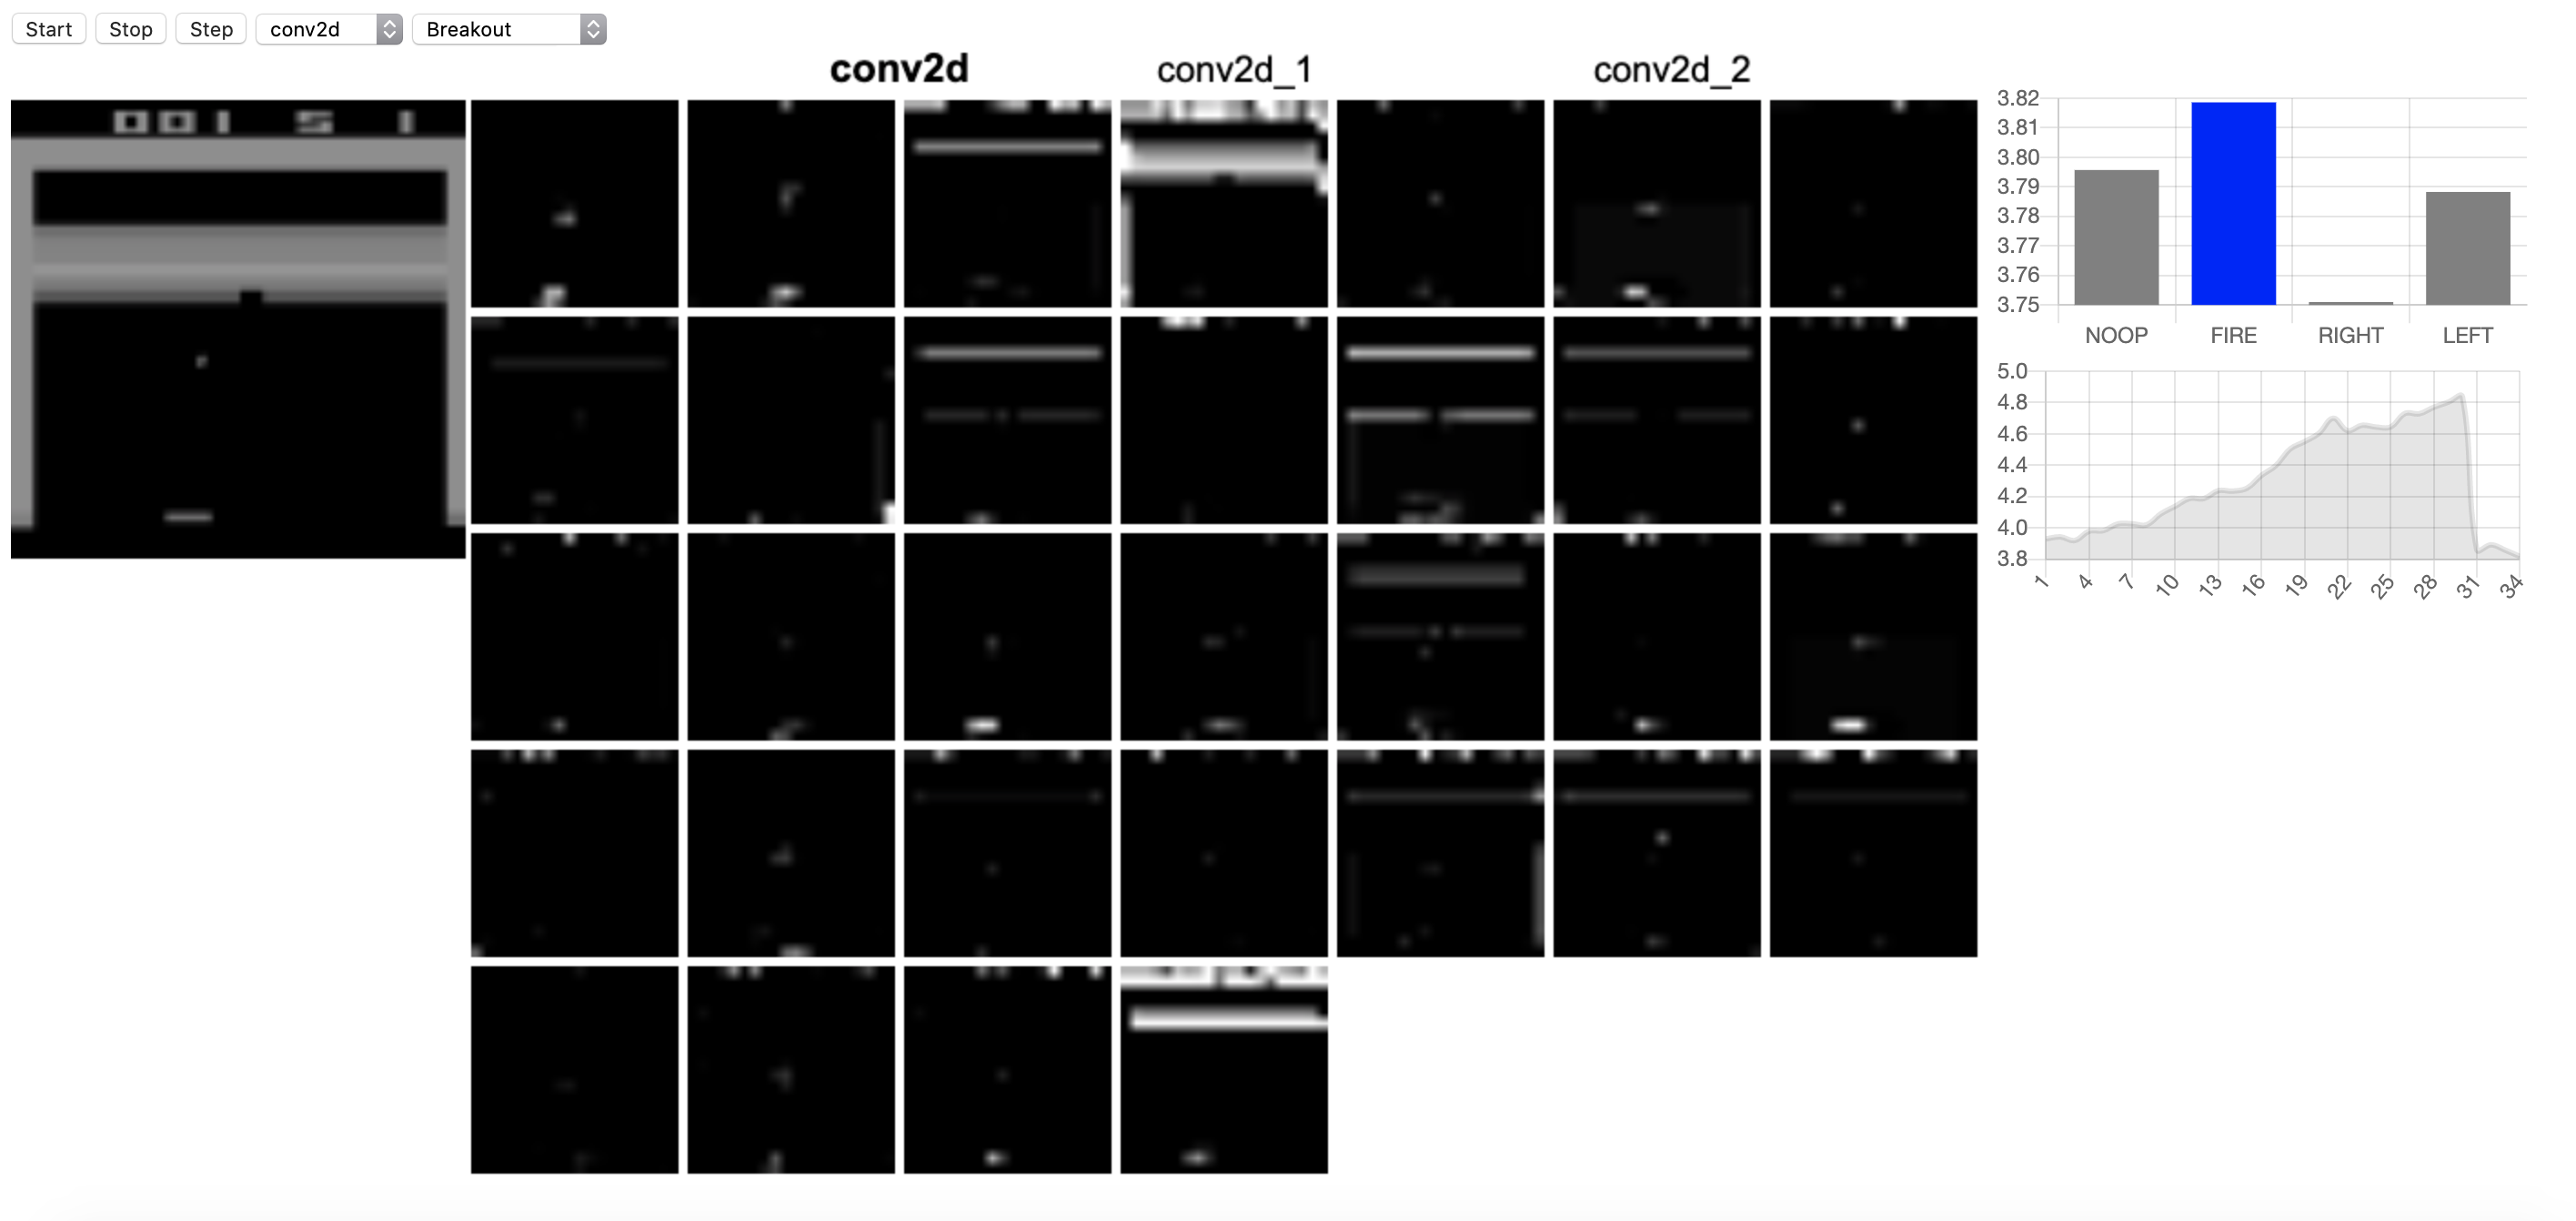
\includegraphics[width=1.0\textwidth]{chapters/chapter5/images/vis_screen.png}
	\caption[Screenshot of visualisation system]{Screenshot of the visualisation system that allows direct control of the environment by using buttons to step the environment. It also displays the different layers of the convolutional neural network and finally we plot both the predicted maximum Q-values at each timestep and the predicted action for the input state.
		\label{fig:vis_system_screenshot}
	}
\end{figure}